\documentclass[12pt]{article}
\usepackage[utf8]{inputenc}
\usepackage[russian]{babel}
\usepackage{graphicx}
\usepackage{listings}
\usepackage{indentfirst}
\usepackage{color}
\usepackage{multirow}
\usepackage{amsmath}
\usepackage{bm}

\definecolor{dkgreen}{rgb}{0,0.6,0}
\definecolor{gray}{rgb}{0.5,0.5,0.5}
\definecolor{ltgray}{rgb}{0.95,0.95,0.95}
\definecolor{mauve}{rgb}{0.58,0,0.82}
\newcommand{\rot}{\mathop{\rm rot}\nolimits}
\renewcommand{\lstlistingname}{Листинг}
\lstset{ %
  language=Python,                % the language of the code
  basicstyle=\footnotesize\ttfamily,           % the size of the fonts that are used for the code
%  numbers=left,                   % where to put the line-numbers
%  numberstyle=\tiny\color{gray},  % the style that is used for the line-numbers
%  stepnumber=2,                   % the step between two line-numbers. If it's 1, each line 
                                  % will be numbered
%  numbersep=5pt,                  % how far the line-numbers are from the code
  backgroundcolor=\color{ltgray},      % choose the background color. You must add \usepackage{color}
  showspaces=false,               % show spaces adding particular underscores
  showstringspaces=false,         % underline spaces within strings
  showtabs=false,                 % show tabs within strings adding particular underscores
  %frame=single,                   % adds a frame around the code
  rulecolor=\color{black},        % if not set, the frame-color may be changed on line-breaks within not-black text (e.g. comments (green here))
  columns=fixed,
  tabsize=2,                      % sets default tabsize to 2 spaces
  captionpos=b,                   % sets the caption-position to bottom
  breaklines=true,                % sets automatic line breaking
  breakatwhitespace=false,        % sets if automatic breaks should only happen at whitespace
%  caption=Valalala,                   % show the filename of files included with \lstinputlisting;
                                  % also try caption instead of title
  keywordstyle=\color{blue},          % keyword style
  commentstyle=\color{gray},       % comment style
  stringstyle=\color{dkgreen},         % string literal style
  escapeinside={\%*}{*)},            % if you want to add LaTeX within your code
  morekeywords={*,...},              % if you want to add more keywords to the set
  deletekeywords={...}              % if you want to delete keywords from the given language
}


\title{Численное сравнение схем расщепления для нестационарного уравнения Стокса}
\author{Борисов В.С.}

\begin{document}

\maketitle

\begin{abstract}
Рассматривается применение схем расщепления для нестационарного уравнения Стокса, которое описывает течение сильно вязкой несжимаемой жидкости. 
%Исходная система связывает в одном уравнение переменные скорости и давления, что при использовании метода конечных элементов, увеличивает количество одновременно решаемых неизвестных. 
Исходная система уравнений включает в себя уравнения для давления и скорости, для решения которой необходимо строить общую матрицу. 
Для сокращения размера матрицы можно применять схемы расщепления, позволяющие расщепить исходную систему связанных уравнений на два раздельных уравнения. Что позволит существенно сократить время счета. Заметим, что подобное расщепление влияет на точность получаемого решения.
%Путем расщепления неизвестные скорости и давления вычисляются по отдельности, то есть вместо составления матрицы включающей обе неизвестные, используются меньшие размером матрицы. При этом изменяется погрешность и время вычисления численного решения.
\end{abstract}

\section{Математическая модель}
Нестационарное уравнение Стокса, описывает течение несжимаемой жидкости в области $\Omega$ с границей $\partial \Omega$:
\begin{equation}
\begin{aligned}
\frac{\partial {\bm u}}{\partial t} -\Delta {\bm u} + \nabla p &= {\bm f}({\bm x}, t), \\
\nabla\cdot{\bm u} &= 0, 
\end{aligned}
\quad {\bm x} \in \Omega, \quad 0<t \leq T,
\end{equation} 
$$
\begin{aligned}
{\bm u(\bm x, t)} &= {\bm g}({\bm x}, t), \quad {\bm x} \in \partial \Omega,\\
{\bm u(\bm x, 0)} &= {\bm u_0}({\bm x}), \quad {\bm x} \in \Omega,
\end{aligned}
\quad 0<t \leq T,
$$
где ${\bm u}({\bm x}, t)$ - скорость, $p({\bm x}, t)$ - давление и ${\bm f}({\bm x}, t)$ - внутренний источник движения. В двумерном случае ${\bm x}=(x_1, x_2)$.

В качестве тестовой модельной задачи, рассчитаем задачу о течении в каверне с подвижной верхней границей. 
Для задания подвижной границы, необходимо задать на ней ненулевые значения скорости.
Задача решается на единичном квадрате $\Omega$ (рис. \ref{fg:cavity}), c границей $\partial \Omega=\Gamma_1 \cup \Gamma_2$. На верхней границе $\Gamma_1$ поставлено условие гладкой стенки $({\bm u}, {\bm n}) = 0$, где ${\bm n}$ нормаль границы и движение идет по направлению границы (направо ${\bm g}({\bm x},t)=(1,0)$). 
В остальной части границы $\Gamma_2=\partial \Omega / \Gamma_1$ поставлено условие прилипания ${\bm g}({\bm x}, t)={\bm 0}$. Внутренние источники скорости отсутствуют ${\bm f}({\bm x}, t)={\bm 0}$. Таким образом, решаемая задача имеет следующую постановку:
\begin{equation}
\begin{aligned}
\frac{\partial {\bm u}}{\partial t} -\Delta {\bm u} + \nabla p &= 0, \\
\nabla\cdot{\bm u} &= 0, 
\end{aligned}
\quad {\bm x} \in \Omega, \quad 0<t \leq T,
\label{eq:scheme-main}
\end{equation} 
с граничными условиями:
\begin{equation}
\begin{split}
{\bm u(\bm x, t)} &= (1, 0), \quad {\bm x} \in \Gamma_1,  \\
{\bm u(\bm x, t)} &= {\bm 0}, \quad {\bm x} \in \Gamma_2, \\
\end{split}
\quad 0<t \leq T,
\label{eq:scheme-boundary}
\end{equation} 
и начальным условием:
\begin{equation}
{\bm u(\bm x, 0)} = {\bm 0}, \quad {\bm x} \in \Omega.
\label{eq:scheme-start}
\end{equation}

\begin{figure}
	\begin{center}
		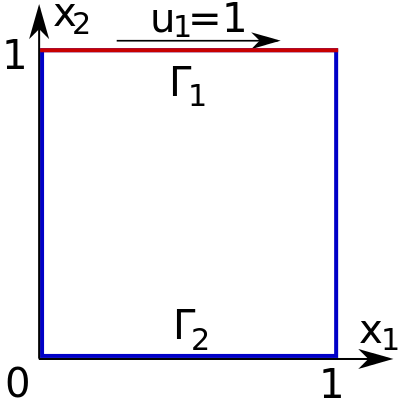
\includegraphics[width=200px]{pics/cavity400}
		\caption{Расчетная область.}
		\label{fg:cavity}
	\end{center}
\end{figure}

\section{Вариационная постановка}
Для численного решения задачи методом конечных элементов, уравнение (\ref{eq:scheme-main}) необходимо привести к вариационной постановке \cite{fenicsbook-2012}. Введем следующие функциональные пространства:
$$
V=\{ ({\bm u}, p) : \, {\bm u} \in H(\mathrm{div}, \Omega), \, p \in L^2(\Omega),  {\bm u}|_{\partial \Omega}=g \},
$$
$$
\hat V=\{ ({\bm v}, q) : \, {\bm v} \in H(\mathrm{div}, \Omega), \, q \in L^2(\Omega), \, {\bm v}|_{\partial \Omega}=0 \},
$$
где $H$ --- пространство Соболева, $L^2$ --- гильбертово пространство.
Умножим уравнения (\ref{eq:scheme-main}) с неизвестными функциями $({\bm u}, p) \in V$  на тестовые функции $({\bm v}, q)$ соответственно, и возьмем интеграл по $\Omega$:
$$
\left\{
\begin{aligned}
\int_{\Omega} \frac{\partial {\bm u}}{\partial t} \cdot {\bm v} \,dx - \int_{\Omega} \Delta {\bm u} \cdot {\bm v} \,dx + \int_{\Omega} \nabla p \cdot {\bm v} \,dx = 0, \\
\int_{\Omega} (\nabla \cdot {\bm u}) \cdot q \,dx = 0.
\end{aligned}
\right.
\quad \forall ({\bm v},q) \in \hat V,
$$
Используя формулу Грина, преобразуем уравнение:
$$
\int_{\Omega} \frac{\partial {\bm u}}{\partial t} \cdot {\bm v} \,dx + \int_{\Omega} \nabla {\bm u} \cdot \nabla {\bm v} \,dx - \int_{\partial \Omega} \frac{\partial {\bm u}}{\partial {\bm n}} \cdot {\bm v} \,dS + \int_{\Omega} \nabla p \cdot {\bm v} \,dx = 0,
$$
здесь интеграл по $\partial \Omega$ равен нулю, т.к. функция ${\bm v} | _ {\partial \Omega} = 0$. Поэтому:
$$
\int_{\Omega} \frac{\partial {\bm u}}{\partial t} \cdot {\bm v} \,dx + \int_{\Omega} \nabla {\bm u} \cdot \nabla {\bm v} \,dx - \int_{\Omega} \nabla p \cdot {\bm v} \,dx = 0.
$$
Общая вариационная постановка в смешанном пространстве $V$, найти $({\bm u}, p) \in V$ такие что:
$$
\int_{\Omega} \frac{\partial {\bm u}}{\partial t} \cdot {\bm v} \,dx + \int_{\Omega} \nabla {\bm u} \cdot \nabla {\bm v} \,dx + \int_{\Omega} \nabla p \cdot {\bm v} \,dx = 0, 
$$
$$
\int_{\Omega} (\nabla \cdot {\bm u}) \cdot q \,dx = 0, \quad ({\bm v}, q) \in \hat V.
$$

\section{Обычные схемы}
Ниже приведенные схемы являются обычными в том смысле, что рассматривают задачу как общую систему уравнений. При этом неизвестные скорости и давления вычисляются как единая переменная. Введем равномерную сетку по времени $\omega_t=\{t^n=n\tau, n=\overline{0,N}, \tau N = T \}$, и определим ${\bm u}_h^n={\bm u}({\bm x}, t^n)$ где $t^n=n\tau$. Также введем промежуточное значения ${\bm u}^*={\bm u}_h^{n+\frac{1}{2}}$ между значениями ${\bm u}_h^n$ и ${\bm u}_h^{n+1}$.

\subsection{Чисто неявная схема.} Чисто неявная схема приведена для сравнения точности со схемами расщепления. Найти такие $({\bm u}_h^{n+1}, p_h^{n+1}) \in V$ для задачи:
$$
\frac{1}{\tau} \int_\Omega {\bm u_h^{n+1}} \cdot {\bm v} \, dx + \int_\Omega \nabla {\bm u_h^{n+1}} \cdot \nabla {\bm v} \, dx + \int_\Omega {\bm v} \cdot \nabla p_h^{n+1} \, dx = \frac{1}{\tau} \int_\Omega {\bm u}_h^n \cdot {\bm v} \, dx, 
$$
$$
\int_\Omega q \nabla \cdot {\bm u_h^{n+1}} \, dx = 0, \quad \forall ({\bm v},q) \in \hat V.
$$

\subsection{Схема Кранка-Николсона.} Схема приведена для сравнения точности со схемами расщепления.
$$
\frac{{\bm u}_h^{n+1}-{\bm u}_h^n}{\tau} - \Delta \frac{{\bm u}_h^{n+1}+{\bm u}_h^n}{2}+\nabla \frac{p_h^{n+1}+p_h^n}{2}=0,
$$
$$
\nabla \cdot \frac{{\bm u}_h^{n+1}+{\bm u}_h^{n}}{2}=0.
$$
Ставится задача, найти такие $({\bm u}_h^{n+1}, \gamma) \in V$ для задачи $a(({\bm v},q), ({\bm u}_h^{n+1},\gamma)) = L(({\bm v},q))$ где
%a = 1.0/tau*inner(u, v)*dx + 0.5*inner(grad(u), grad(v))*dx + inner(v, grad(gamma))*dx + q*div(u)*dx
%L = 1.0/tau*inner(u0, v)*dx - 0.5*inner(grad(u0), grad(v))*dx
\begin{eqnarray}
a(({\bm v}, q), ({\bm u}_h^{n+1}, \gamma)) = \frac{1}{\tau} \int_\Omega {\bm u_h^{n+1}} \cdot {\bm v} \, dx + \frac{1}{2} \int_\Omega \nabla {\bm u_h^{n+1}} \cdot \nabla {\bm v} \, dx + \nonumber\\ 
+ \int_\Omega {\bm v} \cdot \nabla \gamma \, dx + \int_\Omega q \nabla \cdot {\bm u_h^{n+1}} \, dx,
\end{eqnarray}
$$
L(({\bm v},q)) = \frac{1}{\tau} \int_\Omega {\bm u}_h^n \cdot {\bm v} \, dx - \frac{1}{2} \int_\Omega \nabla {\bm u}_h^n \cdot \nabla {\bm v} \, dx, \quad \forall ({\bm v},q) \in \hat V.
$$
Сделаем замену переменных:
$$
\gamma = \frac{p_h^{n+1} + p_h^{n}}{2}.
$$
Ставится задача, найти такие $({\bm u}_h^{n+1}, \gamma) \in V$ для задачи:
\begin{eqnarray}
\frac{1}{\tau} \int_\Omega {\bm u_h^{n+1}} \cdot {\bm v} \, dx + \frac{1}{2} \int_\Omega \nabla {\bm u_h^{n+1}} \cdot \nabla {\bm v} \, dx + \int_\Omega {\bm v} \cdot \nabla \gamma \, dx = \nonumber\\  = \frac{1}{\tau} \int_\Omega {\bm u}_h^n \cdot {\bm v} \, dx - \frac{1}{2} \int_\Omega \nabla {\bm u}_h^n \cdot \nabla {\bm v} \, dx,
\end{eqnarray}
$$
\int_\Omega q \nabla \cdot {\bm u_h^{n+1}} \, dx = - \int_\Omega q \nabla \cdot {\bm u_h^{n}} \, dx, \quad \forall ({\bm v},q) \in \hat V.
$$
Находим $p_h^{n+1}$ из задачи:
$$
\int_\Omega p_h^{n+1} q \, dx = \int_\Omega (2\gamma - p_h^{n}) q \, dx, \quad q \in L^2.
$$

\section{Схемы расщепления}
Расщепление производится по временному слагаемому из уравнения (\ref{eq:scheme-main}). Для каждой схемы строится отдельная вариационная постановка с использованием уже введенных пространств, принцип преобразования оператора Лапласа и избавление от интеграла по границе сохраняется.

Введем равномерную сетку по времени $\omega_t=\{t^n=n\tau, n=\overline{0,N}, \tau N = T \}$, и определим ${\bm u}({\bm x},t)^n={\bm u}({\bm x}, t^n)$ где $t^n=n\tau$. Также введем промежуточное значения ${\bm u}^*={\bm u}_h^{n+\frac{1}{2}}$ между значениями ${\bm u}_h^n$ и ${\bm u}_h^{n+1}$.

\subsection{Схема Дугласа-Рекфорда}
Особенность разбиения состоит в уменьшении размера матрицы для СЛАУ. Вместо составления единого смешанного пространства переменных скорости и давления, вычисления проводятся для скорости и давления по отдельности \cite{vabishchevich-1999}. Таким образом, ставится задача найти ${\bm u} \in H$ и $p \in L^2$:
\begin{equation} \label{eq:scheme-douglas-1}
\frac{{\bm u}^{*}-{\bm u}_h^n}{\tau} - \Delta {\bm u}^{*}+{\nabla}p_h^n=0,
\end{equation}
\begin{equation} \label{eq:scheme-douglas-2}
\frac{{\bm u}_h^{n+1}-{\bm u}_h^n}{\tau} - \Delta {\bm u}^{*}+{\nabla}p_h^{n+1}=0,
\end{equation}
\begin{equation} \label{eq:scheme-douglas-3}
\nabla \cdot {\bm u}_h^n = 0.
\end{equation}
Вычисление ${\bm u}_h^{n+1}$ и $p_h^{n+1}$ происходит в несколько этапов:
\begin{enumerate}
\item 
Сперва вычисляется ${\bm u}^*$, для этого умножим уравнение (\ref{eq:scheme-douglas-1}) на функцию $\bm v$ и возьмем интеграл по $\Omega$, используя формулу Грина для преобразования оператора Лапласа:
$$
\frac{1}{\tau}\int_{\Omega} {\bm u}^*\cdot {\bm v} \,dx + \int_{\Omega} \nabla {\bm u}^* \cdot \nabla {\bm v} \,dx = -\int_{\Omega} {\bm v} \cdot \nabla p_h^{n}\, dx + \frac{1}{\tau} \int_{\Omega} {\bm u}_h^{n} \cdot {\bm v} \,dx.
$$
Решается линейная задача $a({\bm v}, {\bm u}^*) = L({\bm v})$, где
$$
a({\bm v}, {\bm u}) = \frac{1}{\tau}\int_{\Omega} {\bm u}^*\cdot {\bm v} \,dx + \int_{\Omega} \nabla {\bm u}^* \cdot \nabla {\bm v} \,dx,
$$
$$
L({\bm v}) = -\int_{\Omega} {\bm v} \cdot \nabla p_h^{n} \,dx + \frac{1}{\tau} \int_{\Omega} {\bm u}_h^{n} \cdot {\bm v} \,dx;
$$
\item 
Вычитаем из (\ref{eq:scheme-douglas-2}) уравнение (\ref{eq:scheme-douglas-1}):
\begin{equation} \label{eq:scheme-douglas-4}
\frac{{\bm u}_h^{n+1}-{\bm u}^*}{\tau} + {\nabla}(p_h^{n+1} - p_h^n )=0.
\end{equation}
Применяем дивергенцию, из равенства ({\ref{eq:scheme-douglas-3}}), первое слагаемое обнуляется:
$$
\Delta \gamma = \frac{1}{\tau} \nabla \cdot u^{*},
$$
где 
$$
\gamma = p_h^{n+1}-p_h^n.
$$
Вычисляем $\gamma$ из задачи $a(q,\gamma)=L(q)$:
$$
a(q, \gamma) = -\int_{\Omega} \nabla \gamma \nabla q \,dx,
$$
$$
L(q) = \frac{1}{\tau} \int_{\Omega} \nabla \cdot {\bm u}^* q \,dx;
$$
\item 
Вычисляем ${\bm u}_h^{n+1}$ из (\ref{eq:scheme-douglas-4}), предварительно преобразовав уравнение в задачу $a({\bm v}, {\bm u}_h^{n+1}) = L({\bm v})$:
$$
a({\bm v}, {\bm u}_h^{n+1}) = \frac{1}{\tau} \int_{\Omega} {\bm u}_h^{n+1} \cdot {\bm v}\,dx,
$$
$$
L({\bm v}) = \frac{1}{\tau} \int_{\Omega} {\bm u}^* \cdot v \,dx - \int_{\Omega} \nabla \gamma \cdot {\bm v} \,dx;
$$
\item 
Находим $p_h^{n+1}$, выполнив обратную замену решим, задачу $a(q,p_h^{n+1})=L(q)$:
$$
a(q, p) = \int_{\Omega} p_h^{n+1} q\,dx,
$$
$$
L(q) = \int_{\Omega} (\gamma + p_h^n) q\,dx.
$$
\end{enumerate}

%Вычисления проводится в три этапа:
%\begin{enumerate}
%\item Вычисляем ${\bm y}^{n+\frac{1}{2}}$ из первого уравнения;
%\item Вычитаем из (\ref{eq:scheme-douglas-2}) уравнение (\ref{eq:scheme-douglas-1}). Получаем уравнение:
%\begin{equation} \label{eq:scheme-douglas-add}
%\frac{{\bm y}^{n+1}-{\bm y}^{n+\frac{1}{2}}}{\tau} + {\cal P}({\bm y}^{n+1}-{\bm y}^{n})=0,
%\end{equation}
%где оператор ${\cal P}$ на самом деле работает с давлением $e$. Возьмем дивергенцию от (\ref{eq:scheme-douglas-add}). Используя условие (\ref{eq:scheme-zerodiv}) избавляемся от ${\bm y}^{n+1}$ и вычисляем $\gamma = e^{n+1}-e^{n}$.
%\item Подставив $\gamma$ в (\ref{eq:scheme-douglas-add}) явно вычислим ${\bm y}^{n+1}$.
%\end{enumerate}
\subsection{Схема Письмана-Рекфорда.} Особенностью схемы является меньший шаг по времени $\tau/2$ и другое использование промежуточного ${\bm u}^*$. Вычисления происходит аналогично схеме Дугласа-Рекфорда.
\begin{equation} \label{eq:scheme-pisman-1}
\frac{{\bm u}_h^{*}-{\bm u}_h^n}{\tau/2} - \Delta {\bm u}^{*}+\nabla p_h^n=0,
\end{equation}
\begin{equation} \label{eq:scheme-pisman-2}
\frac{{\bm u}^{n+1}-{\bm u}^{*}}{\tau/2} - \Delta {\bm u}^{*}+\nabla p_h^{n+1}=0,
\end{equation}
\begin{equation} \label{eq:scheme-pisman-3}
\nabla \cdot {\bm u}_h^n = 0.
\end{equation}
\begin{enumerate}
\item 
Сперва вычисляется ${\bm u}^*$, для этого умножим уравнение (\ref{eq:scheme-pisman-1}) на функцию $\bm v$ и возьмем интеграл по $\Omega$, используя формулу Грина для преобразования оператора Лапласа:
$$
\frac{2}{\tau}\int_{\Omega} {\bm u}^*\cdot {\bm v} \,dx + \int_{\Omega} \nabla {\bm u}^* \cdot \nabla {\bm v} \,dx = -\int_{\Omega} {\bm v} \cdot \nabla p_h^{n}\, dx + \frac{2}{\tau} \int_{\Omega} {\bm u}_h^{n} \cdot {\bm v} \,dx.
$$
Решается линейная задача $a({\bm v}, {\bm u}^*) = L({\bm v})$, где
$$
a({\bm v}, {\bm u}) = \frac{2}{\tau}\int_{\Omega} {\bm u}^*\cdot {\bm v} \,dx + \int_{\Omega} \nabla {\bm u}^* \cdot \nabla {\bm v} \,dx,
$$
$$
L({\bm v}) = -\int_{\Omega} {\bm v} \cdot \nabla p_h^{n} \,dx + \frac{2}{\tau} \int_{\Omega} {\bm u}_h^{n} \cdot {\bm v} \,dx;
$$
\item 
Вычитаем из (\ref{eq:scheme-pisman-2}) уравнение (\ref{eq:scheme-pisman-1}):
\begin{equation} \label{eq:scheme-pisman-4}
\frac{{\bm u}_h^{n+1}-2{\bm u}^* + {\bm u}_h^{n}}{\tau / 2} + {\nabla}(p_h^{n+1} - p_h^n )=0.
\end{equation}
Применяем дивергенцию, из равенства ({\ref{eq:scheme-pisman-3}}), слагаемые ${\bm u}_h^n$ и ${\bm u}_h^{n+1}$  обнуляются:
$$
\Delta \gamma = \frac{4}{\tau} \nabla \cdot u^{*},
$$
где 
$$
\gamma = p_h^{n+1}-p_h^n.
$$
Вычисляем $\gamma$ из задачи $a(q,\gamma)=L(q)$:
$$
a(q, \gamma) = -\int_{\Omega} \nabla \gamma \nabla q \,dx,
$$
$$
L(q) = \frac{4}{\tau} \int_{\Omega} \nabla \cdot {\bm u}^* q \,dx;
$$
\item 
Вычисляем ${\bm u}_h^{n+1}$ из (\ref{eq:scheme-pisman-4}), предварительно преобразовав уравнение в задачу $a({\bm v}, {\bm u}_h^{n+1}) = L({\bm v})$:
$$
a({\bm v}, {\bm u}_h^{n+1}) = \int_{\Omega} {\bm u}_h^{n+1} \cdot {\bm v}\,dx,
$$
$$
L({\bm v}) = 2 \int_{\Omega} {\bm u}^* \cdot v \,dx - \int_{\Omega} {\bm u}_h^n \cdot v \,dx - \frac{\tau}{2} \int_{\Omega} \nabla \gamma \cdot {\bm v} \,dx;
$$
\item 
Находим $p_h^{n+1}$, выполнив обратную замену решим, задачу $a(q,p_h^{n+1})=L(q)$:
$$
a(q, p) = \int_{\Omega} p_h^{n+1} q\,dx,
$$
$$
L(q) = \int_{\Omega} (\gamma + p_h^n) q\,dx.
$$
\end{enumerate}


\subsection{Покомпонентная схема.} Расщепление происходит по физическим компонентам. Так в первое уравнение для скорости, а второе для давления. Вычисления происходит аналогично схеме Дугласа-Рекфорда.
\begin{equation} \label{eq:scheme-comp-1}
\frac{{\bm u}_h^{*}-{\bm u}_h^n}{\tau} - \Delta{\bm u}^{*}=0,
\end{equation} 
\begin{equation} \label{eq:scheme-comp-2}
\frac{{\bm u}_h^{n+1}-{\bm u}_h^{*}}{\tau} + \nabla p_h^{n+1}=0,
\end{equation}
\begin{equation} \label{eq:scheme-comp-3}
\nabla \cdot {\bm u}_h^n = 0.
\end{equation}
\begin{enumerate}
\item 
Сперва вычисляется ${\bm u}^*$, для этого умножим уравнение (\ref{eq:scheme-comp-1}) на функцию $\bm v$ и возьмем интеграл по $\Omega$, используя формулу Грина для преобразования оператора Лапласа:
$$
\frac{1}{\tau}\int_{\Omega} {\bm u}^*\cdot {\bm v} \,dx + \int_{\Omega} \nabla {\bm u}^* \cdot \nabla {\bm v} \,dx = \frac{1}{\tau} \int_{\Omega} {\bm u}_h^{n} \cdot {\bm v} \,dx.
$$
Решается линейная задача $a({\bm v}, {\bm u}^*) = L({\bm v})$, где
$$
a({\bm v}, {\bm u}) = \frac{1}{\tau}\int_{\Omega} {\bm u}^*\cdot {\bm v} \,dx + \int_{\Omega} \nabla {\bm u}^* \cdot \nabla {\bm v} \,dx,
$$
$$
L({\bm v}) = -\int_{\Omega} {\bm v} \cdot \nabla p_h^{n} \,dx + \frac{1}{\tau} \int_{\Omega} {\bm u}_h^{n} \cdot {\bm v} \,dx;
$$
\item 
Применим дивергенцию к уравнению (\ref{eq:scheme-comp-2}), по уравнению (\ref{eq:scheme-comp-3}) слагаемое ${\bm u}_h^{n+1}$ обнуляется. Вычислим $p_h^{n+1}$ из $a(q, p_h^{n+1})=L(q)$:
$$
a(q, p_h^{n+1}) = \int_{\Omega} \nabla p_h^{n+1} \nabla q \,dx,
$$
$$
L(q) = \frac{1}{\tau} \int_{\Omega} \nabla \cdot {\bm u}^* q \,dx;
$$
\item 
Вычисляем ${\bm u}_h^{n+1}$ из (\ref{eq:scheme-comp-2}), предварительно преобразовав уравнение в задачу $a({\bm v}, {\bm u}_h^{n+1}) = L({\bm v})$:
$$
a({\bm v}, {\bm u}_h^{n+1}) = \int_{\Omega} {\bm u}_h^{n+1} \cdot {\bm v}\,dx,
$$
$$
L({\bm v}) = \int_{\Omega} {\bm u}^* \cdot v \,dx - \tau \int_{\Omega} \nabla p_h^{n+1} \cdot {\bm v} \,dx;
$$
\end{enumerate}

\section{Численное сравнение}
Проведено численное сравнение каждой схемы, на $4$ сетках  с разными размерами $N = 20, 40, 80, 160$, где $N$ это количество узлов на ребре единичного квадрата (рис. \ref{fg:scheme-mesh}). Шаг по времени $\tau = 0.01, 0.005, 0.0025$. Расчетное время $T=0.2$.

\begin{figure}
	\begin{center}
		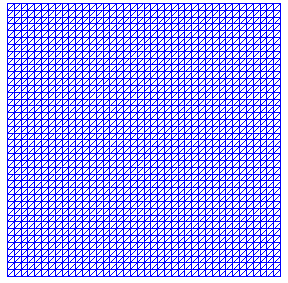
\includegraphics[width=200px]{pics/mesh}
		\caption{Сетка размером $N=40$.}
		\label{fg:scheme-mesh}
	\end{center}
\end{figure}


Для сравнения нормы погрешности вычисляется ``псевдоточное'' решение ${\bm u}_{ex}^n$, на чисто неявной схеме (\ref{eq:scheme-impl-1}), на сетке размером $N=200$ и $\tau=0.00125$.


Вычисление нормы $L_2(\Omega)$ погрешности $\varepsilon^n$ для временного слоя $n$:
$$
\varepsilon^n = \sqrt{\int_{\Omega} ({\bm u}_h^n - {\bm u}_{ex}^n )^2 \, dx}.
$$

На рис. (\ref{fg:scheme-L2-1}) - (\ref{fg:scheme-L2-4}) представлены графики сравнения норм погрешности $L_2(\Omega)$  для четырех разных сеток (по горизонтальной оси временные слои, по вертикальной оси норма погрешности). Обозначения схем на рисунках:
\begin{itemize}
\item cn - схема Кранка-Николсона,
\item dr - схема Дугласа-Рекфорда,
\item im - чисто неявная схема,
\item ct - покомпонентная схема,
\item pr - схема Письмана-Рекфорда.
\end{itemize}



Схемы расщепления проигрывают по точности чисто неявной и Кранка-Николсона, при этом  схема Письмена-Рекфорда неустойчива на сетке $N=20$ независимо от $\tau$. При увеличении размера сетки схема Дугласа-Рекфорда заметно приближается к неявной и Кранка-Николсона.

График на рис. (\ref{fg:scheme-time}) показывает, что время вычисления по схемам расщепления быстрее чем по неявной и Кранка-Николсона. Таким образом схема Дугласа-Рекфорда наиболее предпочтительная для решения задач данного типа.

\begin{figure}
	\begin{center}
		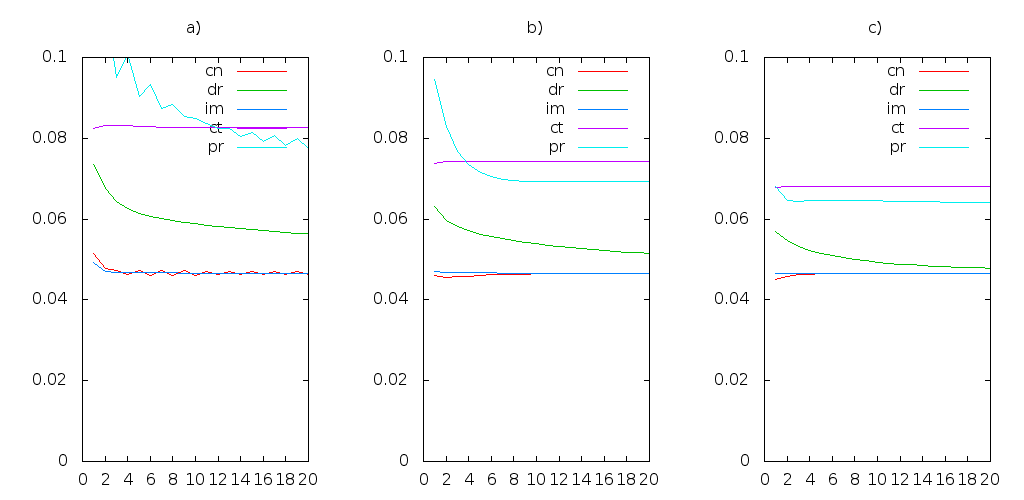
\includegraphics[width=400px]{data160/error_1}
		\caption{Норма погрешности скорости в $L_2$ для $N=20$, a) $\tau=0.01$, b) $\tau=0.005$, c) $\tau=0.0025$.}
		\label{fg:scheme-L2-1}
	\end{center}
\end{figure}

\begin{figure}
	\begin{center}
		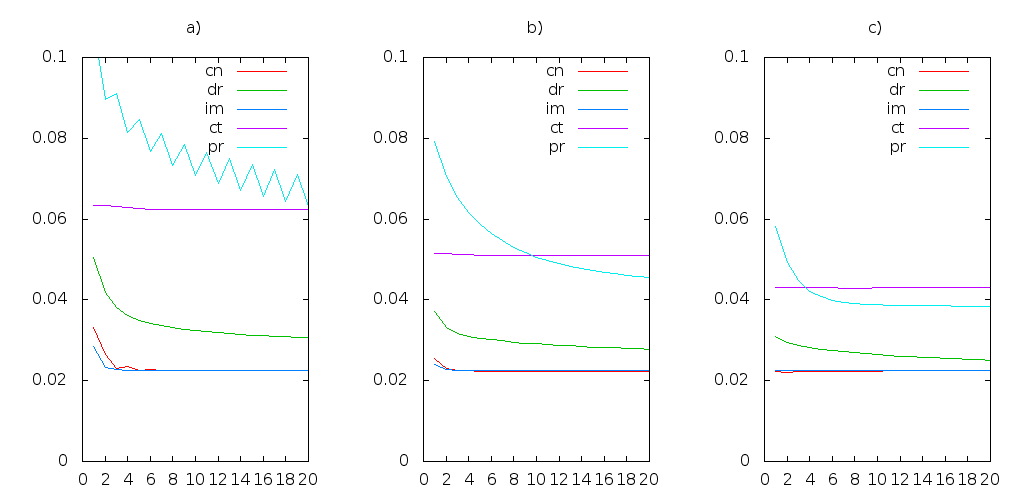
\includegraphics[width=400px]{data160/error_2}
		\caption{Норма погрешности скорости в $L_2$ для $N=40$, a) $\tau=0.01$, b) $\tau=0.005$, c) $\tau=0.0025$.}
		\label{fg:scheme-L2-2}
	\end{center}
\end{figure}

\begin{figure}
	\begin{center}
		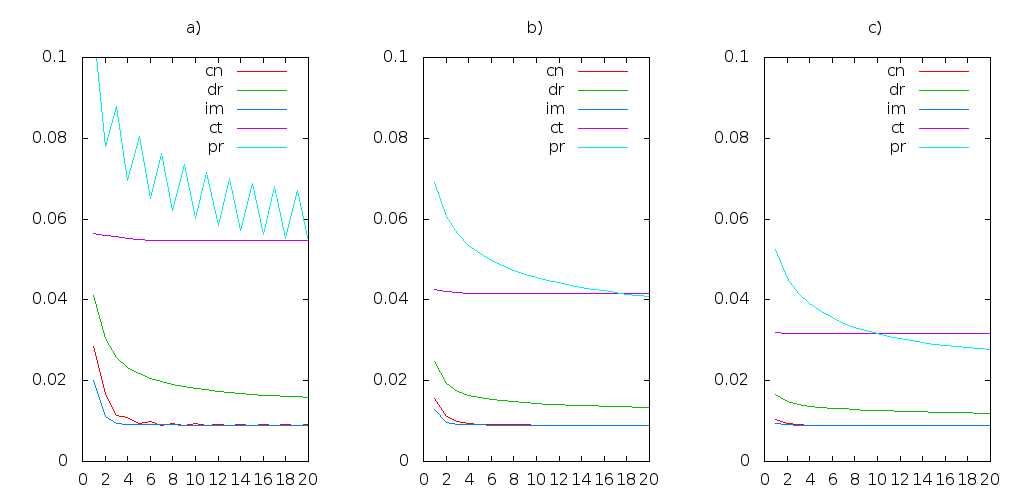
\includegraphics[width=400px]{data160/error_3}
		\caption{Норма погрешности скорости в $L_2$ для $N=80$, a) $\tau=0.01$, b) $\tau=0.005$, c) $\tau=0.0025$.}
		\label{fg:scheme-L2-3}
	\end{center}
\end{figure}

\begin{figure}
	\begin{center}
		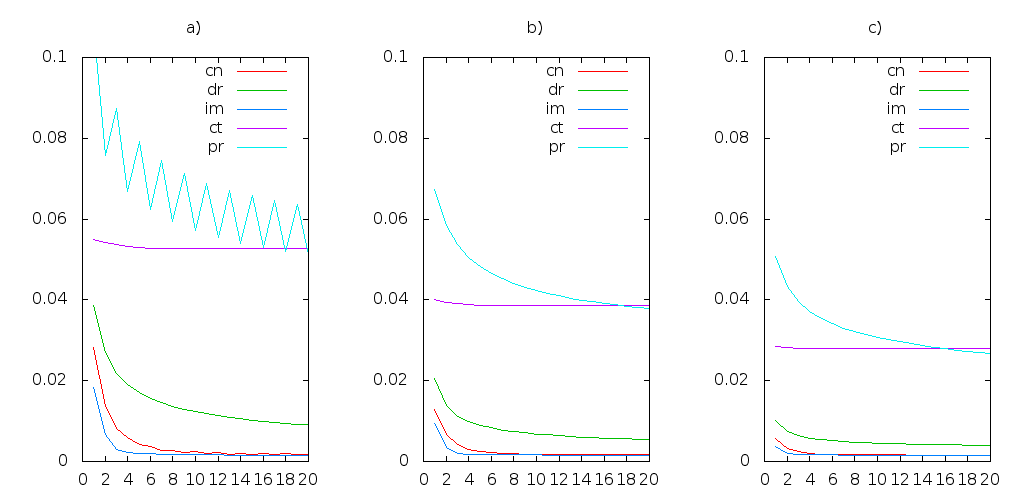
\includegraphics[width=400px]{data160/error_4}
		\caption{Норма погрешности скорости в $L_2$ для $N=160$, a) $\tau=0.01$, b) $\tau=0.005$, c) $\tau=0.0025$.}
		\label{fg:scheme-L2-4}
	\end{center}
\end{figure}

\begin{figure}
	\begin{center}
		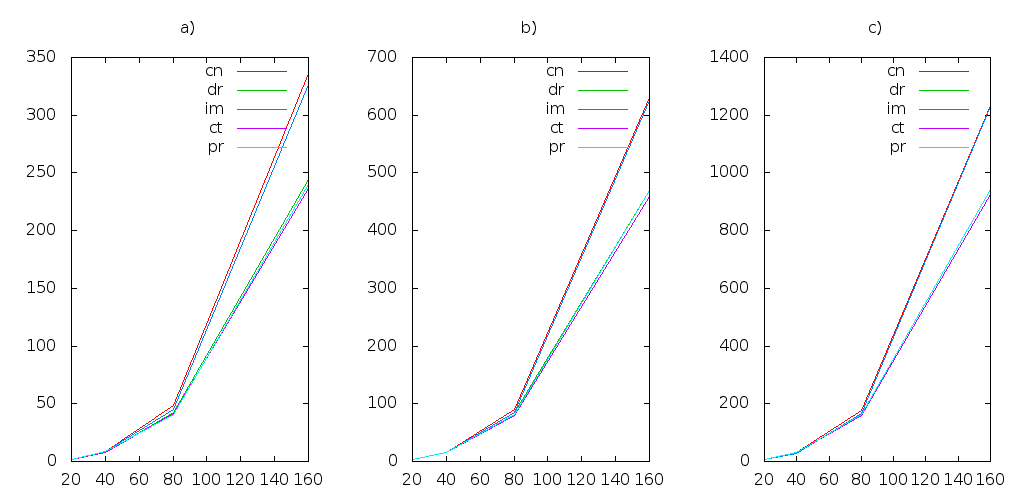
\includegraphics[width=400px]{data160/scheme-time}
		\caption{Время вычисления для a) $\tau=0.01$, b) $\tau=0.005$, c) $\tau=0.0025$.}
		\label{fg:scheme-time}
	\end{center}
\end{figure}

\begin{thebibliography}{9}
\bibitem{vabishchevich-1999} Самарский А.А., Вабищевич П.Н. Аддитивные схемы для задач математической физики. \newblock --- М.: Наука, 1999. 319~с.
\bibitem{fenicsbook-2012} Anders Logg, Kent-Andre Mardal, Garth Wells. Automated Solution of Differential Equations by the Finite Element Method. \newblock --- Berlin: Springer Berlin Heidelberg, 2012. 723~p.
\end{thebibliography}

\end{document}